\documentclass[letterpaper,12pt]{article}
\usepackage{fancyhdr}
\usepackage{amsmath}
\usepackage{amssymb}
\usepackage{bm}
\usepackage{numprint}
\usepackage[margin=1in]{geometry}
\usepackage{graphicx}
% Random packages from
% http://tex.stackexchange.com/questions/50070/landscape-figure-in-latex
% Necessary for sideways pictures
\usepackage{wrapfig}
\usepackage{lscape}
\usepackage{rotating}
\usepackage{epstopdf}
\usepackage{tablefootnote}
% for word wrap verbatim
\usepackage{listings}
\lstset{
   breaklines=true,
   basicstyle=\ttfamily}
% \pagestyle{fancy}
% \lhead{Jesse Mu}
% \rhead{CSCI339 Term Project}
\graphicspath{ {../figures/} }
% Or this, if run from main folder
% \graphicspath{ {./figures/} }



\begin{document}

\title{Cluster Analysis: Identifying Parkinson's Disease Subtypes}
\date{Wednesday, June 10}
\author{Jesse Mu}
\maketitle

\section{Preprocessing}

\subsection{Dataset Description}
951 subjects, 145 metrics, collected 15-4-2012. From Pablo Martinez Mart\'in.
170 subjects with missing values (brought down to 781); these were removed
automatically, even if the missing values were not included in the selected
features below. This will need to be changed later on, by keeping those
removed that still have all selected features and perhaps with some
compensation for missing values.

\subsection{Selected Features}

Combination of non-motor scale (NMS) symptoms and standard motor symptoms.

\begin{table}[ht]
  \centering
  \begin{tabular}{l|l|l|l}
    Name & Type & Format & Description \\
    \hline
    nms\_d1 & byte & \%8.0g & cardiovascular \\
    nms\_d2 & byte & \%8.0g & sleep/fatigue \\
    nms\_d3 & byte & \%8.0g & mood/cognition \\
    nms\_d4 & byte & \%8.0g & percep/hallucinations \\
    nms\_d5 & byte & \%8.0g & attention/memory \\
    nms\_d6 & byte & \%8.0g & gastrointestinal \\
    nms\_d7 & byte & \%8.0g & urinary \\
    nms\_d8 & byte & \%8.0g & sexual function \\
    nms\_d9 & byte & \%8.0g & miscellaneous \\
    tremor & float & \%9.0g & tremor \\
    bradykin & float & \%9.0g & bradykinesia\tablefootnote{Impaired ability to
    adjust the body's position.} \\
    rigidity & float & \%9.0g & rigidity \\
    axial & float & \%9.0g & axial\tablefootnote{Issues affecting the middle of
    the body.} \\
    pigd & float & \%9.0g & postural instability and gait difficulty \\
  \end{tabular}
  \caption{Selected Features and Details}
  \label{tab:selected-features}
\end{table}

\begin{table}[ht]
  \centering
  \begin{tabular}{l|l|l|l}
  Name  &       $\mu$ & $\sigma$ & min-max \\
         \hline
nms\_d1&   1.76&  3.32&   0-24 \\
nms\_d2&   8.71&  8.76&   0-48 \\
nms\_d3&   8.70& 11.83&   0-60 \\
nms\_d4&   1.65&  3.94&   0-33 \\
nms\_d5&   5.22&  7.44&   0-36 \\
nms\_d6&   5.67&  6.92&   0-36 \\
nms\_d7&   8.02&  9.09&   0-36 \\
nms\_d8&   3.57&  5.97&   0-24 \\
nms\_d9&   6.99&  7.74&   0-48 \\
tremor&   2.59&  2.63&   0-12 \\
bradykin& 2.49&  1.39&   0-6 \\
rigidity& 2.34&  1.36&   0-6 \\
axial&    3.28&  2.75&   0-12 \\
pigd&     3.36&  2.77&   0-12 \\
  \end{tabular}
  \caption{Descriptive Statistics}
  \label{tab:descriptive-statistics}
\end{table}

\subsection{Dimensionality Reduction: PCA}

May not be useful? If we're trying to identify \emph{clinically} relevant
features, merging them may not be a good idea.

\begin{figure}[ht]
  \centering
  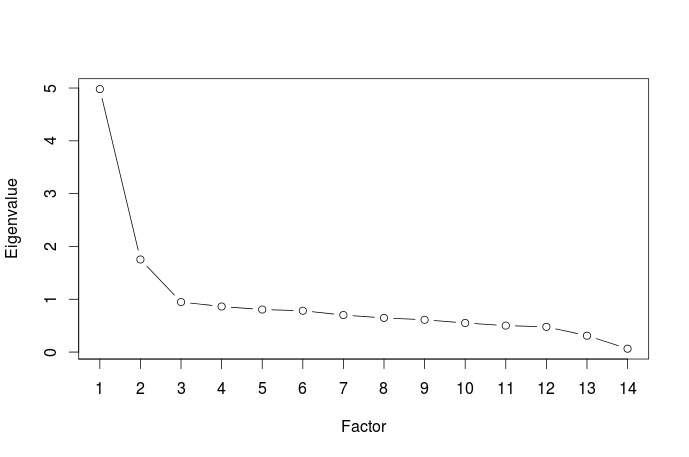
\includegraphics[width=0.8\linewidth]{pca-eigenvalues.png}
  \caption{Scree test: eigenvalues by factor}
  \label{fig:pca-eigenvalues}
\end{figure}

Figure~\ref{fig:pca-eigenvalues} shows scree test elbow occurs around 2 or 3. Also, eigenvalues 1 and $2 > 1$, while 3
is around .9

\section{$k$-means}
\subsection{Identifying optimal number of clusters}

\subsubsection{WSS Error Scree Test}

\begin{figure}[ht]
  \centering
  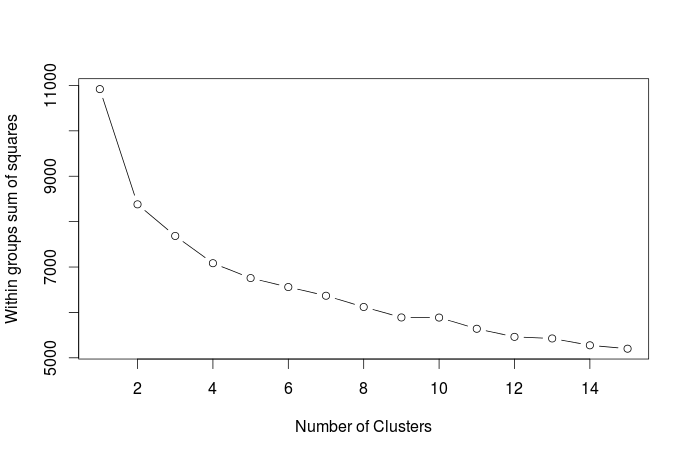
\includegraphics[width=0.8\linewidth]{kmeans-wss-error.png}
  \caption{Scree test: WSS error by cluster size}
  \label{fig:kmeans-wss-error}
\end{figure}

Figure~\ref{fig:kmeans-wss-error} shows no optimal elbow in scree test! Maybe 2-3?

\subsubsection{Gap Statistic}

Optimal cluster is the local maximum of the gap statistic, but it appears to be
consistently increasing in Figure~\ref{fig:gap-statistic}.

\begin{figure}[ht]
  \centering
  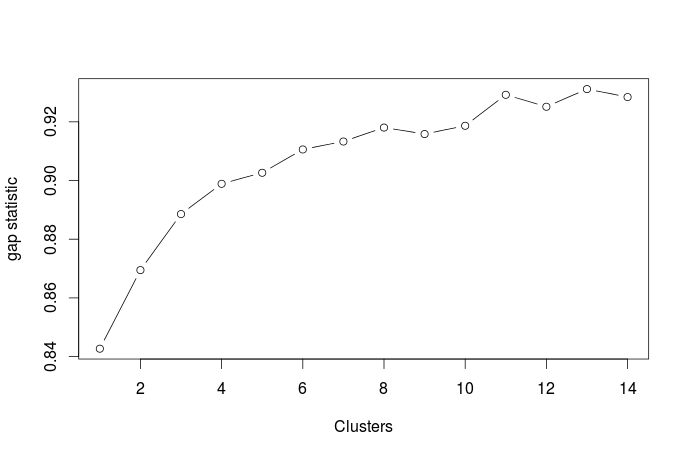
\includegraphics[width=0.8\linewidth]{gap-statistic.png}
  \caption{Gap statistic by cluster size}
  \label{fig:gap-statistic}
\end{figure}

\subsubsection{Average Silhouette Width}

Figure~\ref{fig:asw} shows average silhouette width as being consistently under
0.25 for all clusters, implying the data is not well structured.

\begin{figure}[ht]
  \centering
  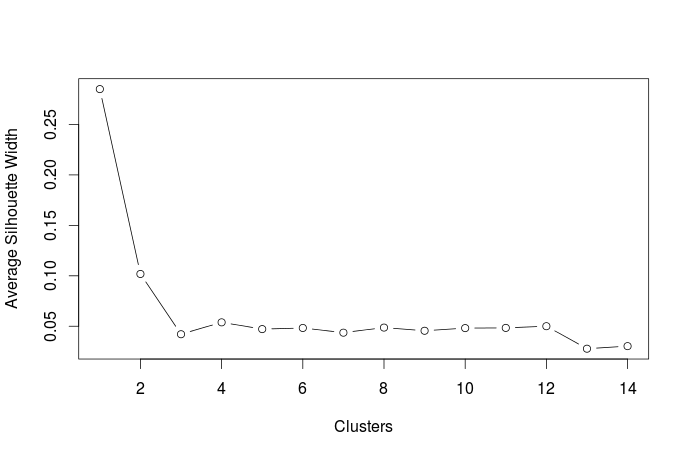
\includegraphics[width=0.8\linewidth]{asw.png}
  \caption{Average silhouette width by cluster size}
  \label{fig:asw}
\end{figure}

% \subsubsection{\texttt{NbClust} package}

\subsection{Cluster statistics}
% CLUSTERS: 2
% ================================
% Sizes: 201 580
% WithinSS: 4248.585 4132.434
% Sum WithinSS: 8381.019
% CLUSTERS: 3
% ================================
% Sizes: 420 231 130
% WithinSS: 2618.368 1973.82 3076.542
% Sum WithinSS: 7668.73
% CLUSTERS: 4
% ================================
% Sizes: 61 372 145 203
% WithinSS: 1481.25 1845.389 2147.988 1609.555
% Sum WithinSS: 7084.183
\begin{table}[ht]
  \centering
  \begin{tabular}{l|l|l|l}
    $k$ & $n$ & Within SS & sum(Within SS) \\
    \hline
    2 & 201/580 & 4248.585/4132.434 & 8381.019 \\
    3 & 420/231/130 & 2618.368/1973.82/3076.542 &  7668.73 \\
    4 & 61/372/145/203 & 1481.25/1845.389/2147.988/1609.555 & 7084.183
  \end{tabular}
  \caption{Cluster statistics}
  \label{tab:cluster-statistics}
\end{table}

\subsection{Silhouette plots}

Available in
Figures~\ref{fig:kmeans-silhouette-2},~\ref{fig:kmeans-silhouette-3},
and~\ref{fig:kmeans-silhouette-4}. Note: constructed with standardized
$z$-score data.

\begin{figure}[ht]
  \centering
  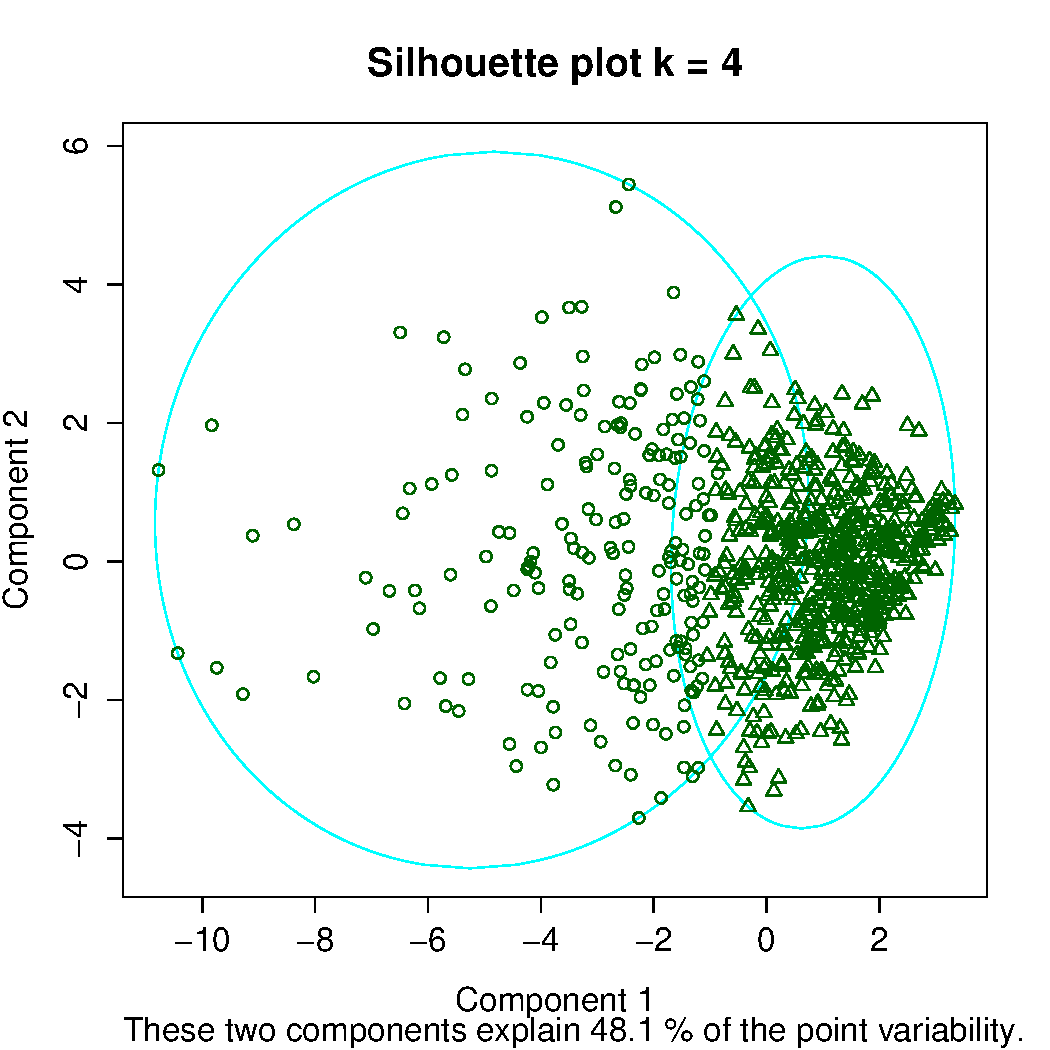
\includegraphics[width=0.8\linewidth]{kmeans-silhouette-2.pdf}
  \caption{$k$-means cluster silhouette plot, $k = 2$}
  \label{fig:kmeans-silhouette-2}
\end{figure}

\begin{figure}[ht]
  \centering
  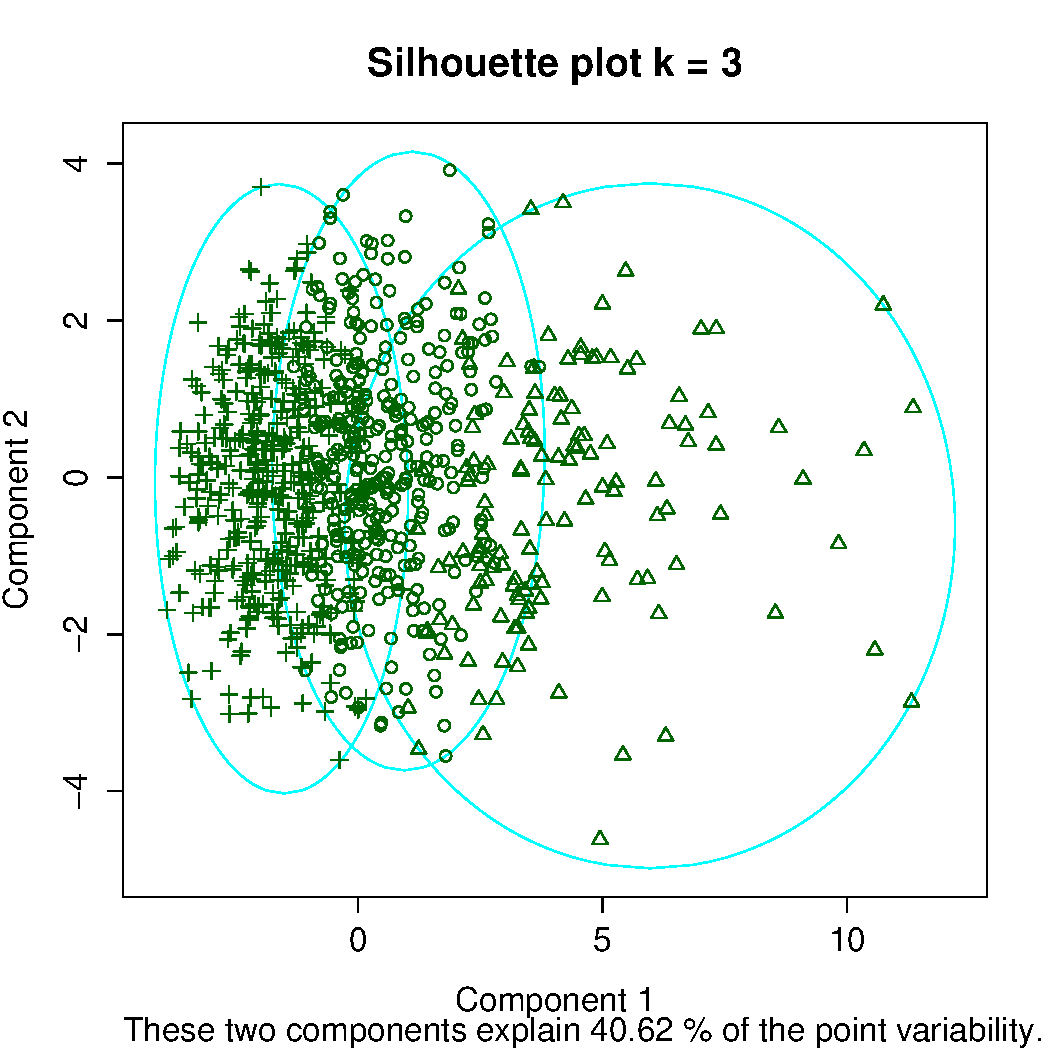
\includegraphics[width=0.8\linewidth]{kmeans-silhouette-3.pdf}
  \caption{$k$-means cluster silhouette plot, $k = 3$}
  \label{fig:kmeans-silhouette-3}
\end{figure}

\begin{figure}[ht]
  \centering
  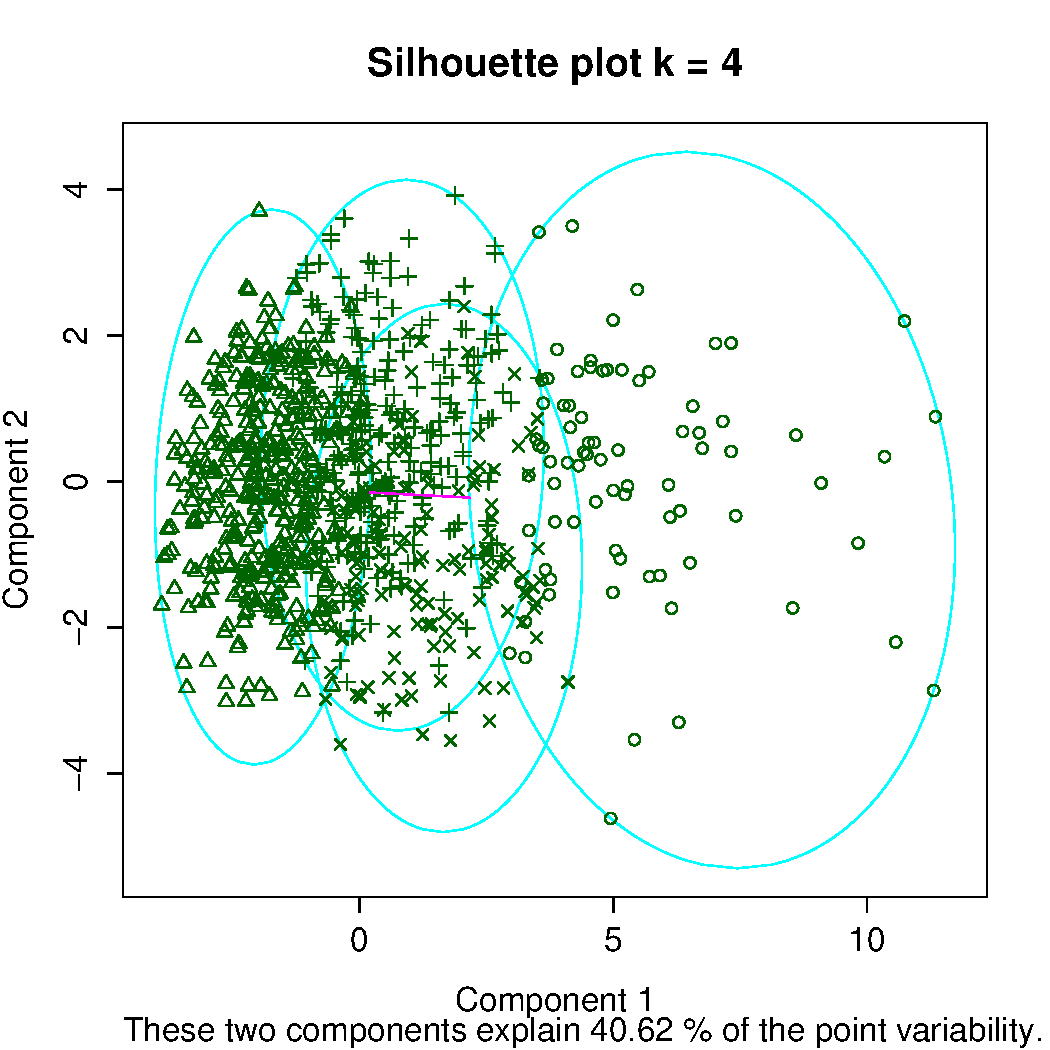
\includegraphics[width=0.8\linewidth]{kmeans-silhouette-4.pdf}
  \caption{$k$-means cluster silhouette plot, $k = 4$}
  \label{fig:kmeans-silhouette-4}
\end{figure}

\subsection{Decision trees based on clusters}
% seed = 911
% CLUSTERS: 2
% ================================
% Complexity Parameter: 0.03482587
% 10-fold CV error: 0.134443
% Root node error: 0.2573624
% CLUSTERS: 3
% ================================
% Complexity Parameter: 0.01
% 10-fold CV error: 0.1946223
% Root node error: 0.4622279
% CLUSTERS: 4
% ================================
% Complexity Parameter: 0.01
% 10-fold CV error: 0.2483995
% Root node error: 0.5236876
\begin{table}[ht]
  \centering
  \begin{tabular}{l|l|l|l|l|l}
    $k$ & CP\tablefootnote{Complexity Parameter} & CV Xerror\tablefootnote{10-fold cross
    validation} & Root Feature &
    Root Error & Figure \\
    \hline
    2 & 0.0348 & 0.134 & axial $\geq$ 0.44 & 0.257 & Figure~\ref{fig:kmeans-dtree-2} \\
    3 & 0.0100 & 0.194 & bradykin $<$ 0.0041 & 0.462 & Figure~\ref{fig:kmeans-dtree-3} \\
    4 & 0.0100 & 0.248 & bradykin $<$ 0.0041 & 0.523 & Figure~\ref{fig:kmeans-dtree-4} \\
  \end{tabular}
  \caption{$k$-kmeans decision trees statistics}
  \label{tab:k-means-dtrees}
\end{table}

\begin{figure}[ht]
  \centering
  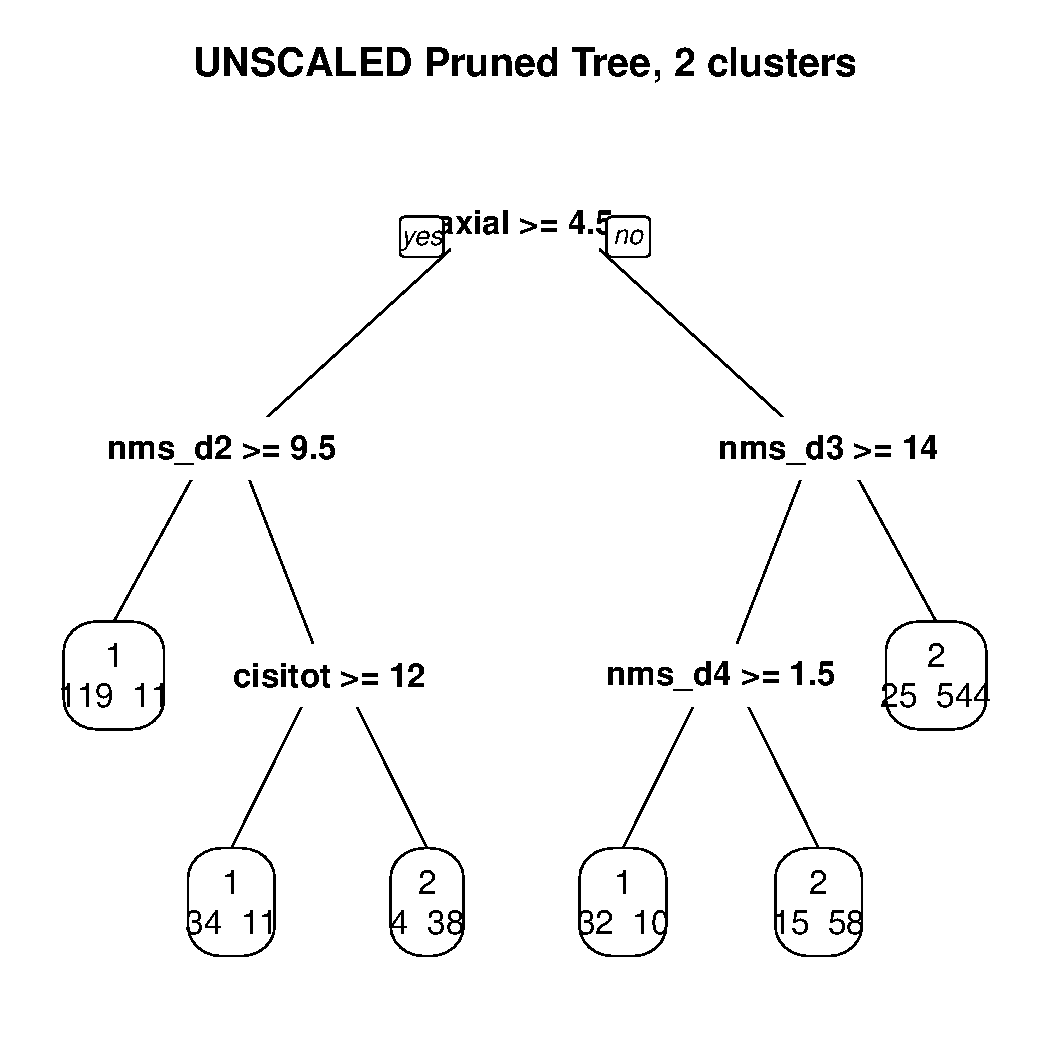
\includegraphics[width=0.8\linewidth]{dtree-kmeans-pruned-unscaled-2.pdf}
  \caption{Decision Tree from $k$-means clustering, 2 clusters}
  \label{fig:kmeans-dtree-2}
\end{figure}

\begin{figure}[ht]
  \centering
  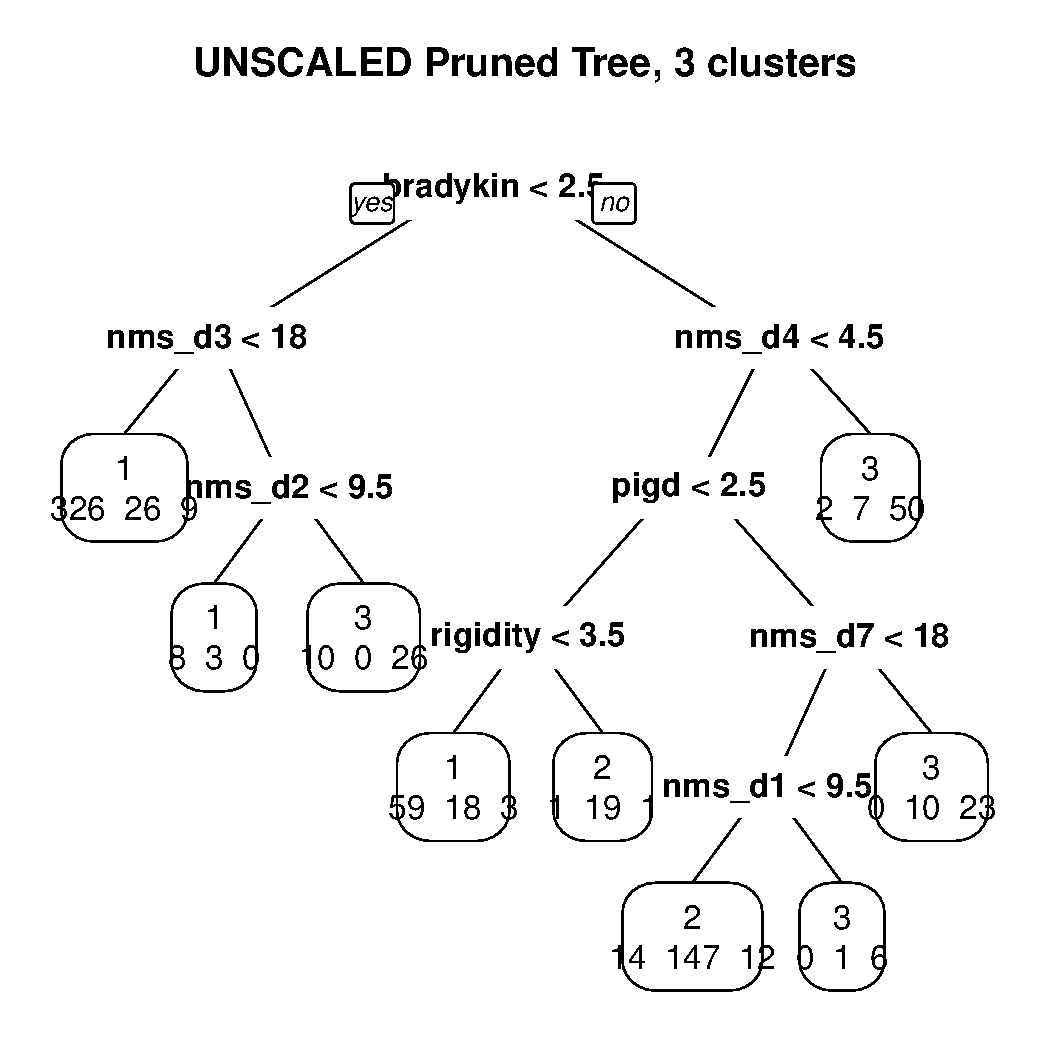
\includegraphics[width=0.8\linewidth]{dtree-kmeans-pruned-unscaled-3.pdf}
  \caption{Decision Tree from $k$-means clustering, 3 clusters}
  \label{fig:kmeans-dtree-3}
\end{figure}

\begin{figure}[ht]
  \centering
  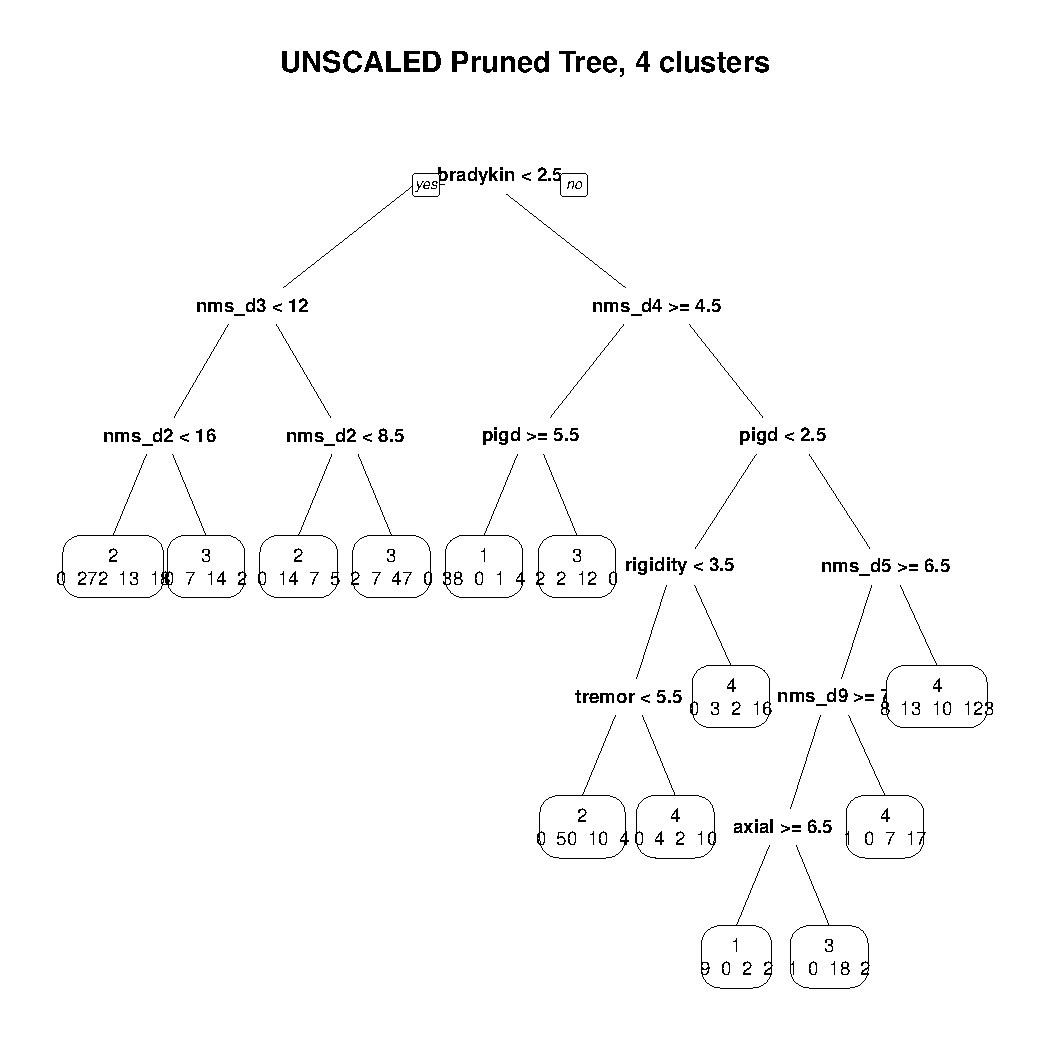
\includegraphics[width=0.8\linewidth]{dtree-kmeans-pruned-unscaled-4.pdf}
  \caption{Decision Tree from $k$-means clustering, 4 clusters}
  \label{fig:kmeans-dtree-4}
\end{figure}

\subsection{Interpretation of Clusters}

\subsubsection{Cluster summaries}

Available in
Figures~\ref{fig:kmeans-summaries-2},~\ref{fig:kmeans-summaries-3},
and~\ref{fig:kmeans-summaries-4}. Error bar is standard error.

\subsubsection{Interpretation}

$k = 2$ seems too basic. Cluster is organized solely by severity - all
symptoms, including motor and nonmotor, are higher in severity in cluster 1,
and lower in cluster 2. Quite consistently, groups in cluster 1 are generally
of slightly higher age and pd duration.

$k = 3$ seems like a further development of $k = 2$, where clusters are simply
organized by linearly increasing severity.

$k = 4$ is where it gets interesting.

\begin{figure}[ht]
  \centering
  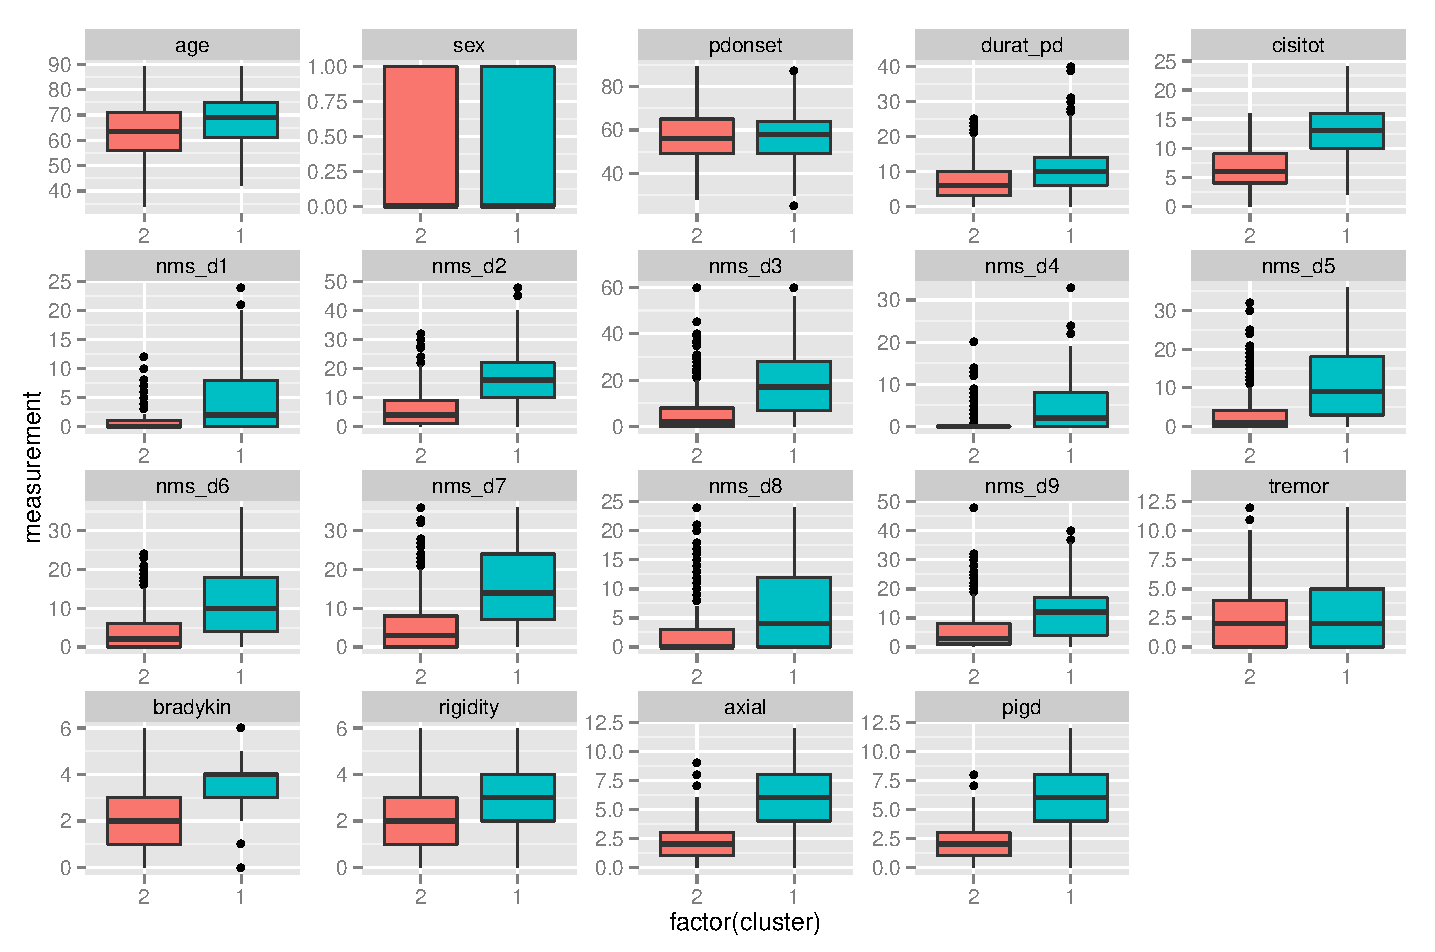
\includegraphics[width=\linewidth]{kmeans-summaries-2.pdf}
  \caption{Cluster Summaries, $k = 2$}
  \label{fig:kmeans-summaries-2}
\end{figure}

\begin{figure}[ht]
  \centering
  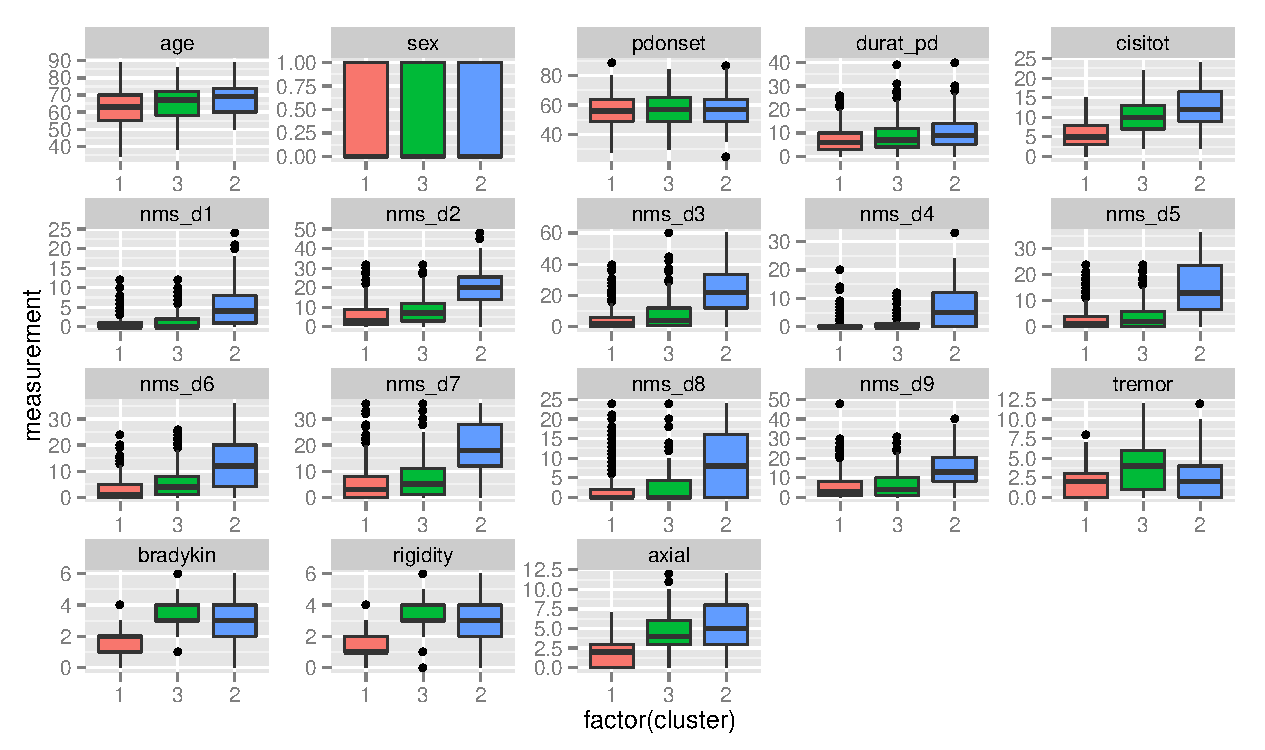
\includegraphics[width=\linewidth]{kmeans-summaries-3.pdf}
  \caption{Cluster Summaries, $k = 3$}
  \label{fig:kmeans-summaries-3}
\end{figure}

\begin{figure}[ht]
  \centering
  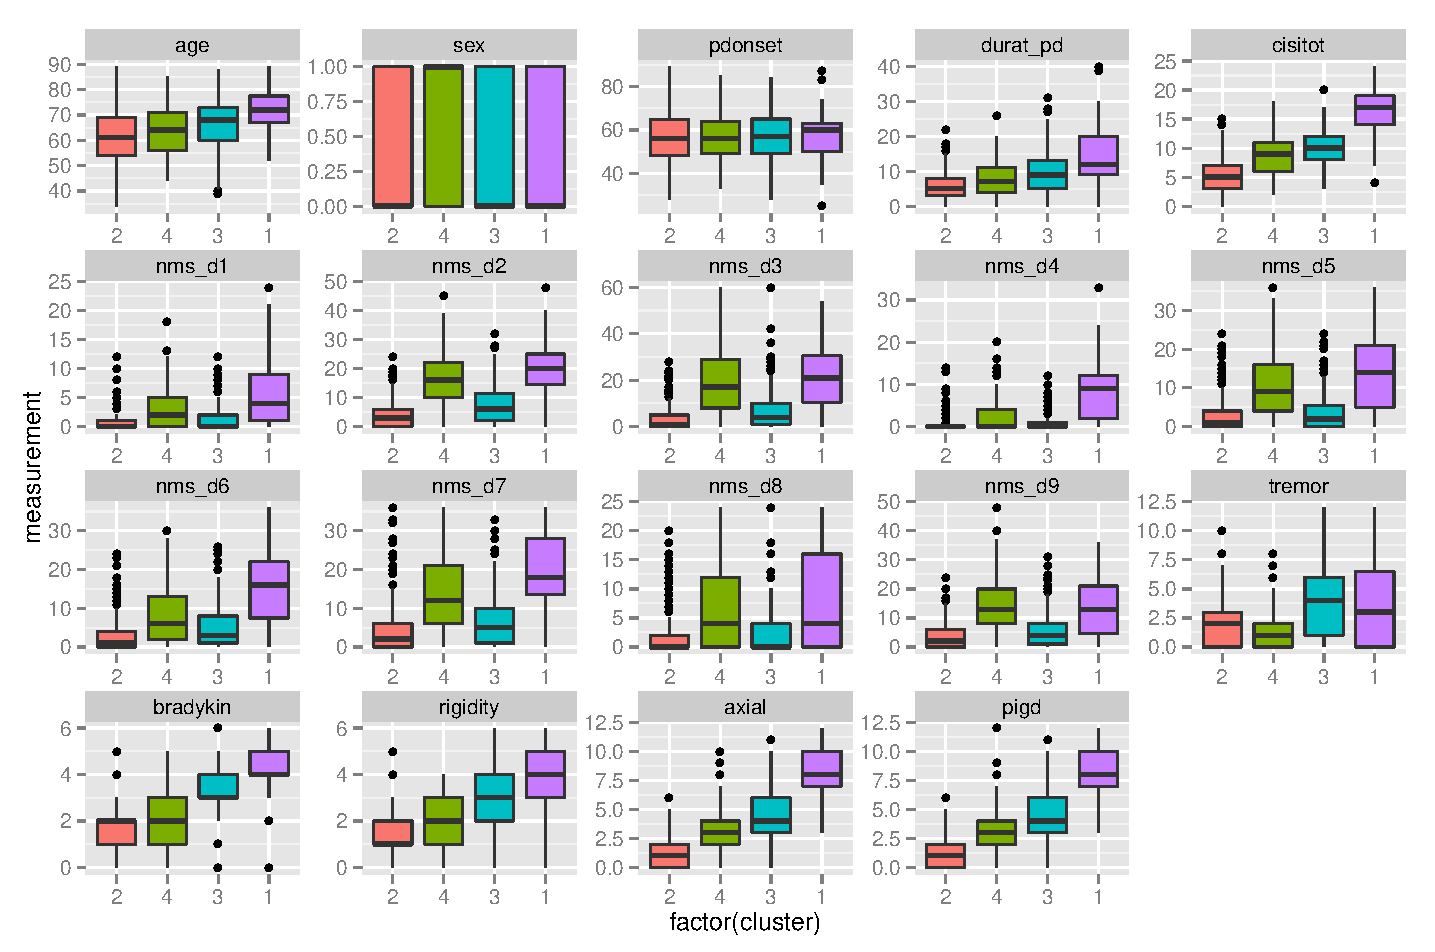
\includegraphics[width=\linewidth]{kmeans-summaries-4.pdf}
  \caption{Cluster Summaries, $k = 4$}
  \label{fig:kmeans-summaries-4}
\end{figure}

\section{Affinity Propagation}

\subsection{Clustering}

AP with input preferences minimized ($q = 0$) resulted in 8 clusters.
With the standard median input preferences ($q = 0.5$), algorithm failed to
converge with default parameters. Even setting damping factor to 0.98, maximum
iterations to 10000, and convergence iterations to 1000 failed to converge.
Might need to try a longer term work.

\emph{However}, given that input preferences control how many clusters are
found, I don't think it's very useful to have some dozen clusters running
around.

\subsubsection{Silhouette Plots}

Silhouette plot in Figure~\ref{fig:ap-silhouette} looks pretty weak, really.
Tons of overlap between the clusters.

\begin{figure}[ht]
  \centering
  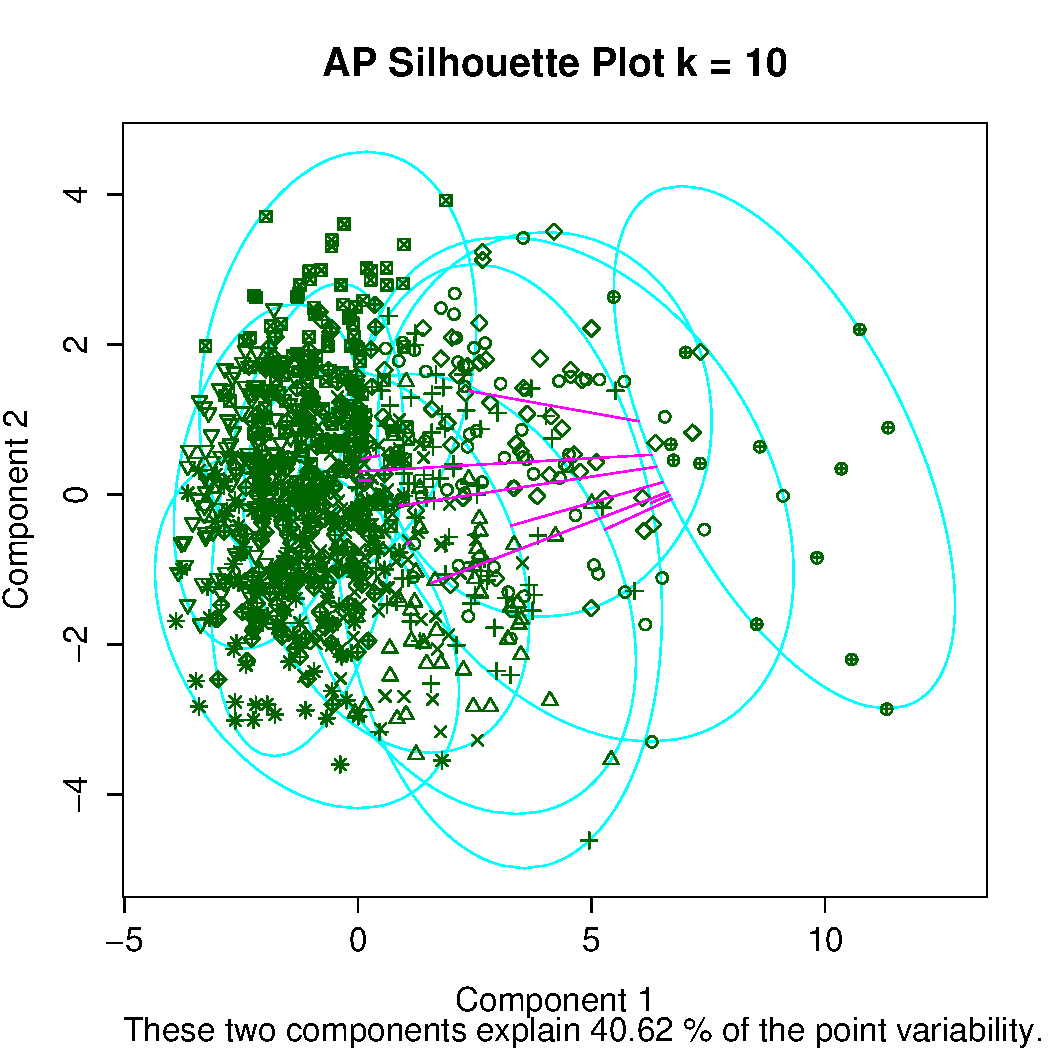
\includegraphics[width=0.8\linewidth]{ap-silhouette.pdf}
  \caption{AP silhouette plot, $k = 8$}
  \label{fig:ap-silhouette}
\end{figure}

\subsection{Interpretation}

Boxplot summary of clusters available in Figure~\ref{fig:ap-summaries}.
\textbf{Discussion forthcoming.}

\begin{figure}[ht]
  \centering
  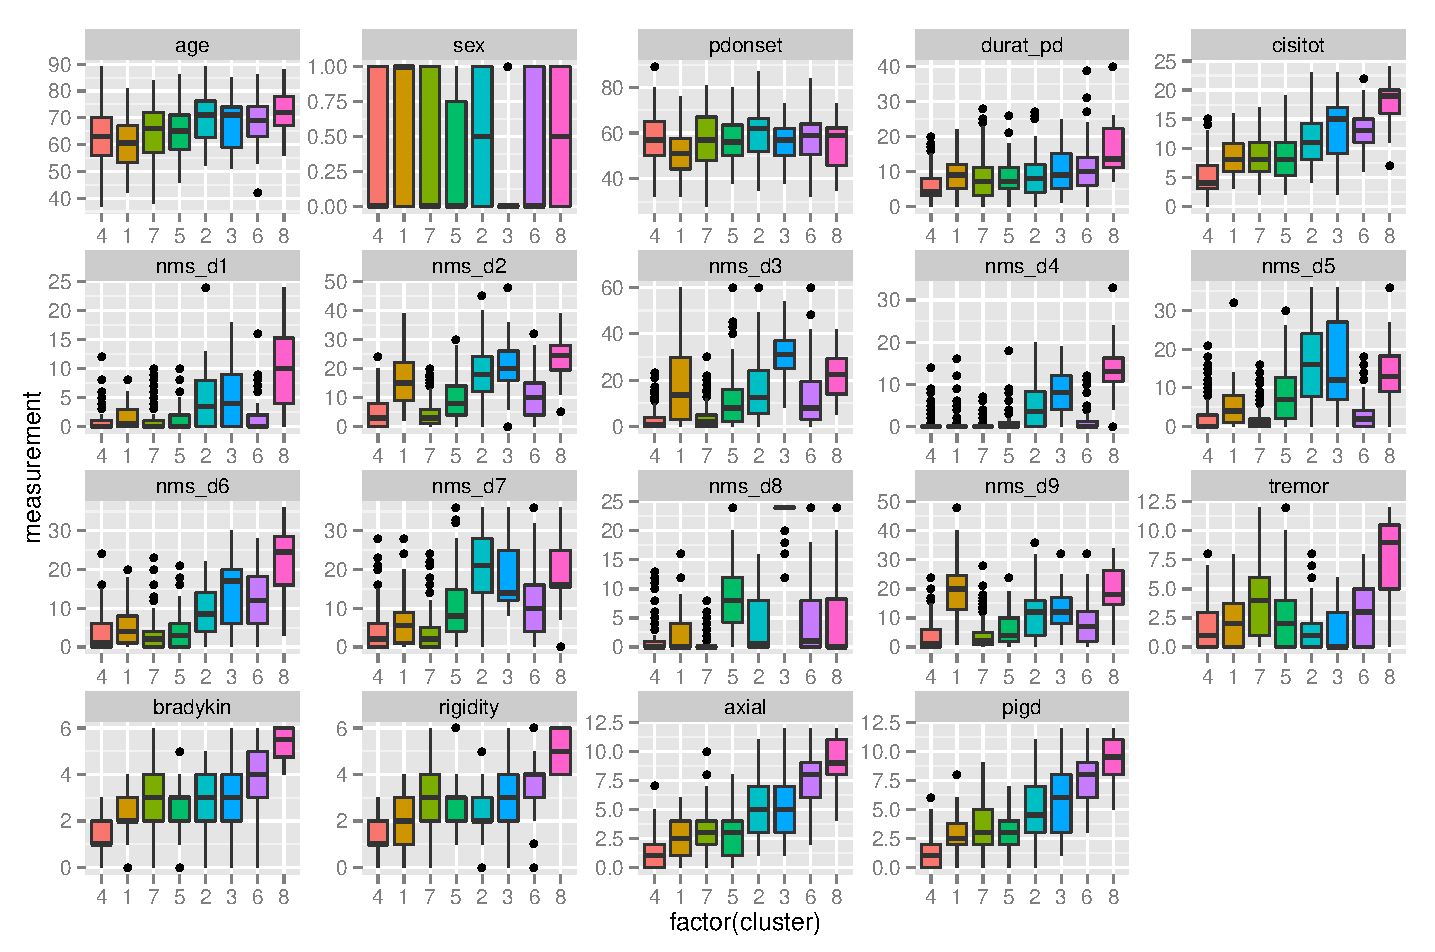
\includegraphics[width=0.8\linewidth]{ap-summaries.pdf}
  \caption{AP Boxplot Summaries}
  \label{fig:ap-summaries}
\end{figure}

\section{Biclustering}

Used BCBimax clustering algorithm. Clusters seem quite sparse.

\begin{figure}[ht]
  \centering
  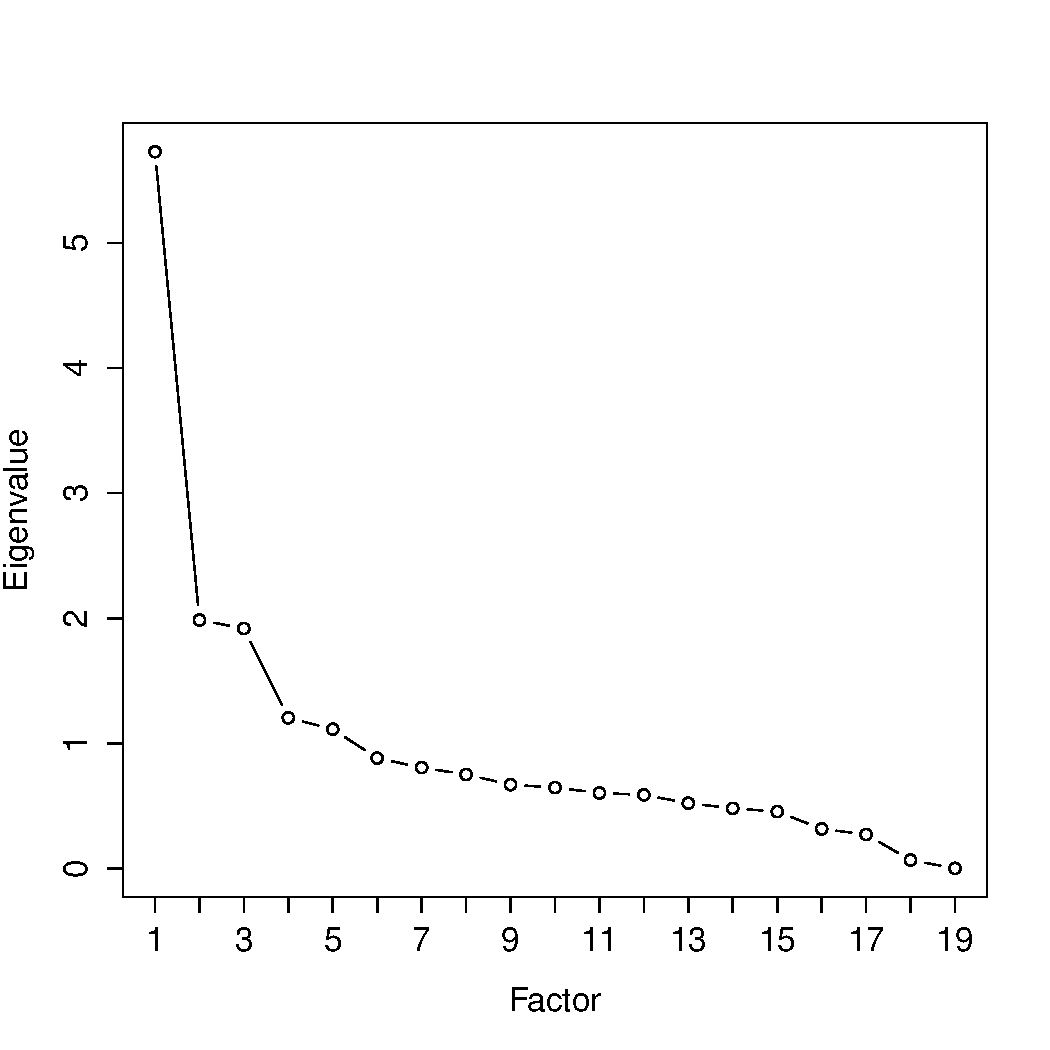
\includegraphics[width=0.8\linewidth]{biclust-16.pdf}
  \caption{Biclustering $N = 16$}
  \label{fig:biclust-16}
\end{figure}

\begin{figure}[ht]
  \centering
  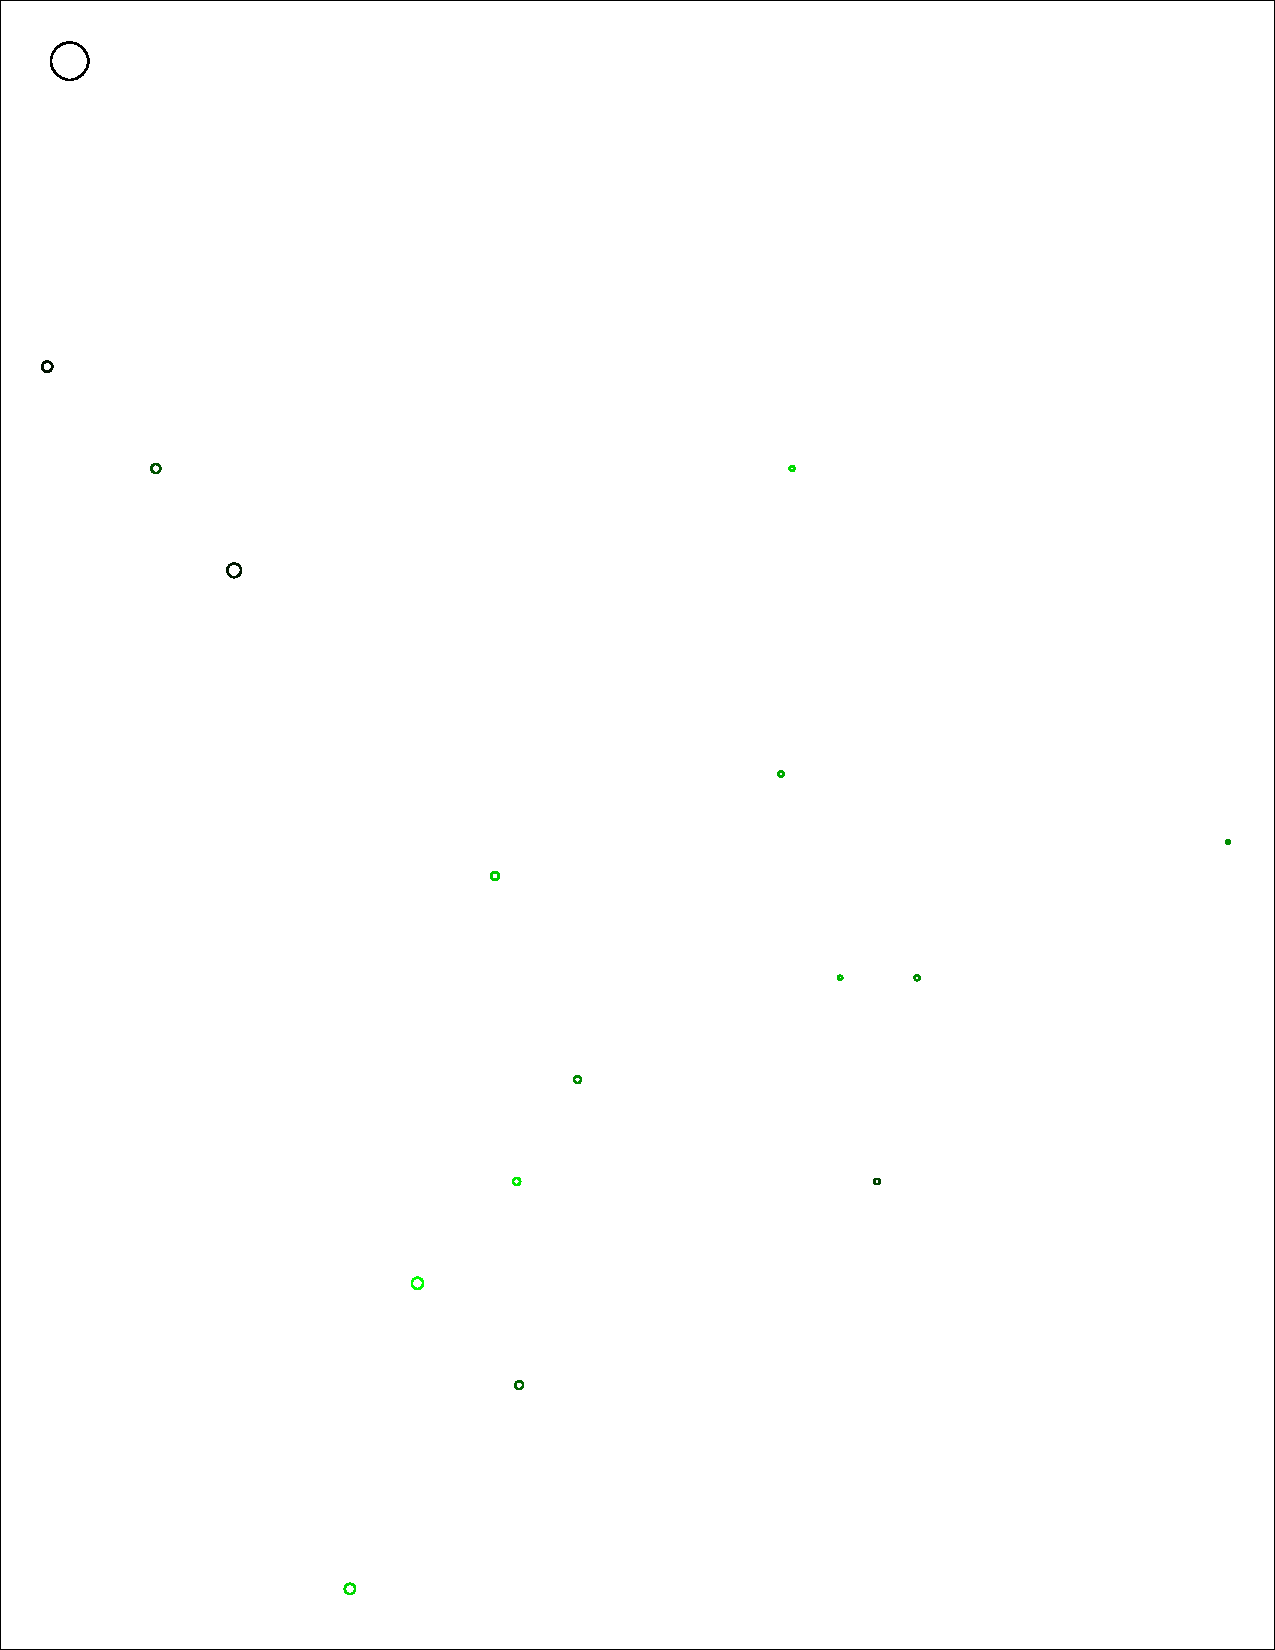
\includegraphics[width=0.8\linewidth]{bubbleplot-16.pdf}
  \caption{Bubbleplot $N = 16$}
  \label{fig:bubbleplot-16}
\end{figure}

\section{Subspace clustering}

% TODO: Wat.

\section{Bayesian Networks}

\end{document}
